\chapter{North Sea Data Collection} \label{ch:NDD}

At this stage, the automatic photo-identification system in development is capable of detecting cetaceans in large panoramic images and post-processing these detections into a form ready for individual identification, as outlined in Chapter \ref{ch:cetDet}. So far, the detector has been trained and tested on data collected by Newcastle University's Marine MEGAfauna Lab whilst researching the abundance of Indo-Pacific bottlenose dolphins (\textit{Tursiops aduncus}) off the coast of Zanzibar, Tanzania \cite{sharpe_indian_2019}. 

Whilst the Marine MEGAfauna Lab research heavily in the Indian Ocean around Zanzibar \cite{yang_description_2020, temple_life-history_2020, temple_marine_2019, temple_marine_2018, weigmann_revision_2020, barrowclift_social_2017}, this is not the only place they operate \cite{temple_by-catch_2021, yang_classification_2017, yang_influence_2022}. In recent years, their work has begun to include more local waters such as the North Sea off the coast of Northumberland, UK \cite{van_bressem_visual_2018, yang_characterization_2021}. These waters are known to host a wide variety of marine mammals, with the Marine MEGAfauna Lab focussing efforts specifically on the bottlenose dolphin (\textit{Tursiops truncatus}) and white-beaked dolphin (\textit{Lagenorhynchus albirostris}) populations. 

Near the end of the Mask R-CNN detection model's completion, the Marine MEGAfauna Lab were preparing to begin a large scale bottlenose and white-beaked abundance estimate and health assessment survey. As such the opportunity arose to validate the detector's generalisability on data which is similar in composition and purpose, however was collected in a different geographic location, at a different time, and containing different species to the data used to train and test the detector.

As a result, this Chapter discusses the collection of abundance estimate data in Northumberland, UK for the purpose of model and technique evaluation as outlined in Chapter \ref{ch:cetDet}. In order to achieve this evaluation, the photo-identification data was curated and transformed from a biological catalogue into a computer vision dataset known as \textit{The Northumberland Dolphin Dataset 2020} (NDD20) - the creation of which will be discussed. The post-processing of NDD20 and additional external data sources to produce a dataset capable of training an individual identification model is also examined. 

\section{Data Collection}\label{ch:NDD,sec:dataCollection}

The following Section provides context for the data collection survey, beginning by briefly outlining the geographic area in which the data was collected and discussion of why the area was chosen. Next the survey effort is discussed in detail, including a run-down of the methodology used, for the purposes of reproducibility. 

\subsection{The Survey Area}\label{ch:NDD,sec:dataCollection,sub:surveyArea}

Data collection was conducted in and around the Coquet to St. Mary's Marine Conservation Zone (MCZ), located off the coast of Northumberland, UK. The MCZ, established in January 2016 through powers granted by the Marine and Coastal Access Act 2009 \cite{noauthor_marine_2009}, covers approximately 40km of coastline from Almouth in the north to Whitley Bay in the south, extending outwards 7.5km at its greatest to cover an area around 192km$^{2}$. A map of the survey area and MCZ can be seen in Figure \ref{fig:survey-map}.

 \begin{figure}
	\begin{center}
		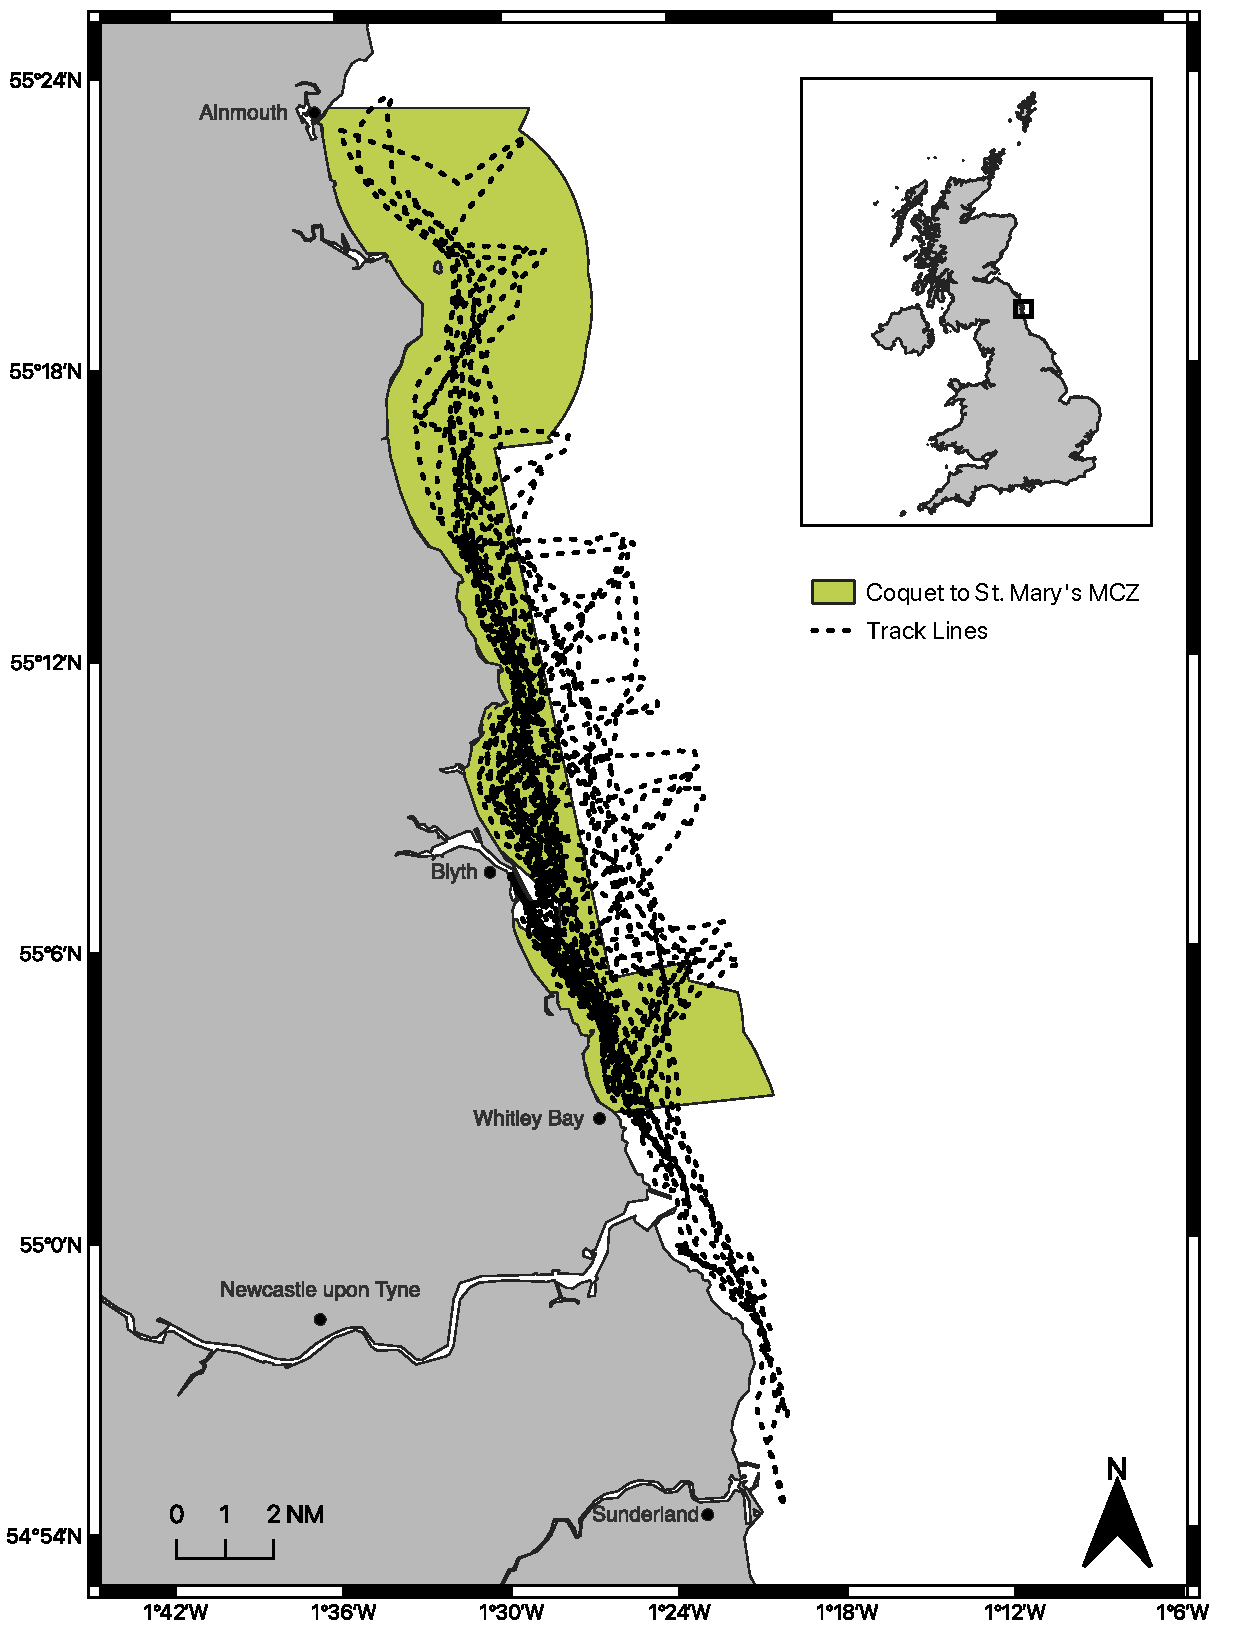
\includegraphics[scale=0.7]{Chapter4/figs/survey_map.pdf}
	\end{center}
	\caption{Map of the survey area, with the Coquet to St. Mary's MCZ highlighted. Track lines for all survey days are overlaid.}
	\label{fig:survey-map}
\end{figure}

The area is of high importance, supporting a wide variety of marine life thanks to sections of intertidal and sub-tidal rock and sediment, making it fertile feeding grounds for the bottlenose and white-beaked dolphins which make use of the area. As a result of this fertility, as well as waters up to 30m deep in some places, the MCZ sees high levels of fishing activity - typically for crustaceans using pots \cite{stephenson_spatial_2017}. Whilst these fishing vessels operate from a number of small ports throughout the North East of England, the MCZ itself lies close to the large Port of Blyth. As a result, the MCZ boundary provides a 250m buffer zone around the limits of the port in order to reduce economic damage. This survey region was selected as no previous surveying had been undertaken in the area for the purposes of cetacean abundance estimates and health assessment.

\subsection{Survey Effort}\label{ch:NDD,sec:dataCollection,sub:surveyEffort}

Dedicated bottlenose and white-beaked dolphin photo-identification surveys were conducted in the MCZ between 19/07/2019 and 10/10/2019, with a total of 27 surveys undertaken. These were performed using a 5.6m rigid inflatable boat (RIB) with a 50 horsepower four-stroke outboard engine. All surveys began from Newcastle University's Blyth Marine Station, located in the Port of Blyth, before entering the MCZ.

Surveys initially began by following set transect lines, traversing between the northern and southern-most points of the MCZ. Thanks to limited success encountering individuals strictly following transect lines however, the survey switched to more opportunistic surveying based on reports from two citizen science groups: the Newbiggin-by-the-Sea Dolphin Watch\footnote{Newbiggin-by-the-Sea Dolphin Watch: \href{https://en-gb.facebook.com/groups/NEWILDDOLPHINMONITORINGPROJECT/}{facebook.com/groups/NEWILDDOLPHINMONITORINGPROJECT}} and the North East Cetacean Project\footnote{North East Cetacean Project: \href{https://en-gb.facebook.com/groups/NorthEastCetaceanProject/about/}{facebook.com/groups/NorthEastCetaceanProject}}. The use of citizen scientists for photo-id surveys has seen increased prevalence in recent years, with multiple studies producing promising results if access to groups of dedicated citizen scientists is available, like in Northumberland \cite{araujo_population_2017, currie_conservation_2018, armstrong_photographic_2019, araujo_photo-id_2019}. Track lines showing movement of the vessel were recorded via GPS tracking, and can be seen in Figure \ref{fig:survey-map}. When dolphins were encountered, the time stamp was recorded alongside other effort data such as direction of travel, sea state, species, group size, and demographic composition.

Surveys were only conducted in Beaufort Sea States $\le 3$ \cite{world_meteorologicial_society_beaufort_1970} without heavy rain. Outside of these conditions surveying can become unsafe and the photographs unusable for photo-id because of swell and lens splash. Due to the nature of the North Sea, conditions outside of these restrictions can be common. Surveying was performed using the constant scanning method \cite{mann_behavioral_1999}, with cues including sight of dorsal fins breaching the waterline, splashing, and leaping. For each survey the vessel was manned by at least two dedicated observers and a skipper, in line with other photo-id surveys \cite{sharpe_indian_2019, bessesen_lacaziosis-like_2014, silva_winter_2012}.

Individual dolphins in an encounter were photographed randomly using a Canon EOS 550D Digital SLR with a Canon 70–200mm zoom lens, aiming to capture photographic data for every individual present. Camera settings can be found in Appendix \ref{app:DataCollectionCameraSettings}. Multiple photographs were captured of each cetacean over the course of the encounter to ensure identifiable information could be fully captured. When capturing an encounter care was taken not to approach individual cetaceans at an angle less than $30^{\circ}$, keeping as parallel as possible and to speeds no greater than 6 knots in order to prevent the cetaceans becoming stressed or injured as per Marine Management Organisation guidelines. All members of the survey team were trained in minimising wildlife disturbance through the WiSe Scheme by the Yorkshire Wildlife Trust\footnote{WiSe Scheme: \href{https://www.wisescheme.org/}{wisescheme.org}}, with the survey itself having the approval of Newcastle University's Ethics Board.

\subsection{Field Season Summary}\label{ch:NDD,sec:dataCollection,sub:summary}

Of the 27 days where surveys were conducted 14 contained encounters. Of these, 12 were made up of bottlenose dolphin; only two were made up of white-beaked dolphin. No encounters contained both species. Groups were defined using the 10m chain rule \cite{smolker_sex_1992}. Group size averaged 12 for bottlenose dolphins, typical for the species \cite{shane_ecology_1986}. Altogether 40 individuals were identified and catalogued, broken down into 30 bottlenose and 10 white-beaked dolphins. Of all animals encountered, 27\% were calves. They have been excluded from this analysis as they could not be considered independent due to reliance on their mothers, and had not yet developed permanent markings.

Images collected were processed for use in the photo-identification catalogue as to remove any images with no value, such as those which were out of focus or did not contain any cetacean. Animals present in the images were coded according to their distinctiveness as per the guidelines presented in \cite{urian_recommendations_2015}. Those coded D1 were considered very distinctive with little chance of misidentification, whilst those coded D2 were considered moderately distinctive with small prominent markings which could allow for a high chance of correct classification provided the image is clear. CF coded individuals were those which contained little to no identifying information which have a high chance of misclassification. Once coded, animals considered D1 and D2 were individually identified.

\section{The Northumberland Dolphin Dataset 2020}\label{ch:NDD,sec:NDD20}

The fieldwork season and data processing undertaken resulted in a photo-identification catalogue of bottlenose and white-beaked dolphins currently inhabiting the Coquet to St. Mary's MCZ. Photo-identification catalogues utilised in marine biology however are not in the form required for training or validating a computer vision model. As such, further processing was required to transform the catalogue into a dataset capable of both validating the instance segmentation model developed in Chapter \ref{ch:cetDet}, as well as training a model for fine-grained individual identification. This Section discusses the creation of the Northumberland Dolphin Dataset 2020 (NDD20) \cite{trotter_ndd20_2020}, the computer vision dataset created from the photo-identification catalogue.

\subsection{Above Water Data}\label{ch:NDD,sec:NDD20,sub:aboveWaterData}

During fieldwork 4940 images were collected which contained part of a cetacean above the water line. Of these, 2201 images were considered usable for the creation of NDD20. Issues rending images unusable included a significant amount of water splash obscuring the cetacean, poor lighting conditions, or where individuals in a pod were too close together to accurately determine by eye the outline of all individuals. 

From manual analysis it was determined that not all images contained enough identifying information for individual classification labels. Because of this, the decision was made to include multiple levels of granularity to the dataset. As all images contained part of a cetacean, each one could be labelled to allow for instance segmentation training. To enable this, each mask located was given the label \texttt{dolphin}. Next, masks could be provided a fine-grained species classification. Thanks to the difference in colour between bottlenose and white-beaked dolphins, every mask labelled for instance segmentation could also be provided a species label - either \texttt{BND} or \texttt{WBD} representing bottlenose and white-beaked dolphin respectively. 

At the highest level of granularity, some masks contained enough information to allow for individual identification. If an ID could be attained with high confidence, likely from images with D1 or D2 coded individuals, the mask containing the individual was provided an \texttt{ID} label. Recent work has shown that publicly available datasets containing animals may aid poachers \cite{beery_can_2021}. In response, to protect ongoing cetacean research efforts a pseudo-anonomisation has been performed. This however does not diminish the value of the dataset to computer vision researchers. It is not the case that images with sequential filenames were captured sequentially, and all individual IDs have been randomly allocated a numerical value rather than the code given to them by the Marine MEGAfauna Lab. All EXIF data found in the images has also been removed. The photo-identification catalogue itself is not publicly hosted at this time.

Data was labelled at a pixel level using the VGG Image Annotator \cite{dutta_via_2019} in a similar fashion to the Zanzibar dataset as discussed in Section \ref{ch:cetDet,sec:initialTesting,sub:zanzibar}. In order to speed up the process data labellers were employed through Newcastle University's Jobs On Campus service\footnote{Newcastle University Jobs On Campus: \href{https://www.ncl.ac.uk/careers/jobs/opportunities-on-campus/jobsoc/\#jobsocoverview}{ncl.ac.uk/careers/jobs/opportunities-on-campus/jobsoc/}} to manually annotate the masks and label them for instance segmentation. Once complete all masks were checked for error correcting and consistency purposes. Afterwards, the extra labels for both species and individual level identification were added. As this required expert knowledge, data labellers were not utilised for this. Example above water images from NDD20 and the labels assigned can be seen in Figure \ref{fig:above-water-example}.

\begin{figure}
	\begin{center}
		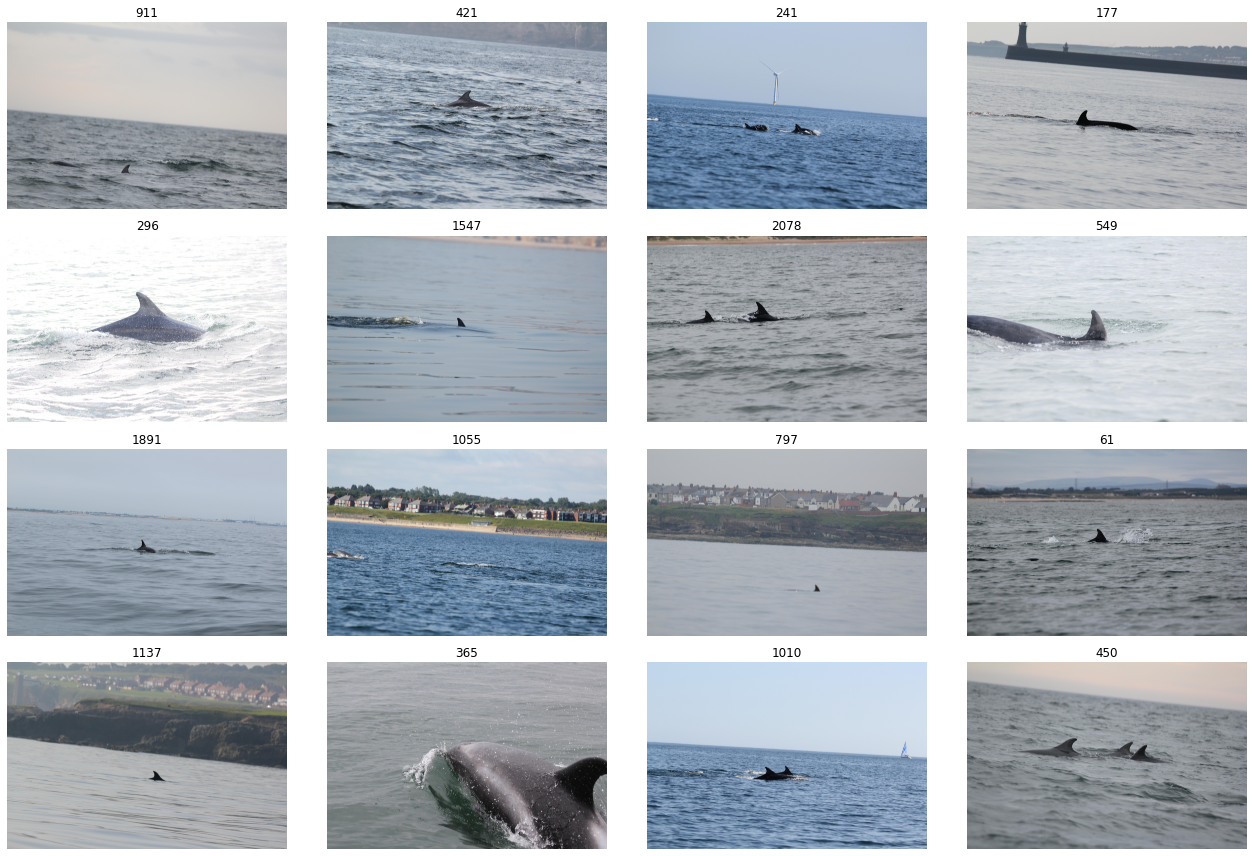
\includegraphics[scale=0.3]{Chapter4/figs/aweg-tiled.png}
	\end{center}
	\caption{Example above water images from NDD20 with filenames displayed. Class labels for masks in each image are noted in Appendix \ref{app:NDD20AwegLabels}.}
	\label{fig:above-water-example}
\end{figure}

\subsection{Below Water Data}\label{ch:NDD,sec:NDD20,sub:belowWaterData}

In addition to the above water imagery captured during fieldwork, NDD20 also contains below water images. Underwater photo-id is not as widely used compared to its above-water counterpart at present, however uses have been noted for certain species and environments in recent years \cite{van_bressem_visual_2018, veronique_underwater_2022}. Whilst this data has not been utilised in the work on automatic photo-id presented in this thesis it is important to discuss all aspects of the dataset created. Images contained in the below water section of NDD20 are a subset of a much larger collection of images produced by the Marine MEGAfauna Lab during work in the Farnes Deep MCZ, a glacial trench situated approximately 11km from the Northumberland coast. Opportunistic surveys undertaken since 2011 have shown the area to contain a high abundance of white-beaked dolphin activity \cite{van_bressem_visual_2018}. Data from these surveys takes the form of screen grabs from high definition video footage captured by a diver using GoPro Hero 3 and Go Pro Hero 4 cameras. 

To mirror the above water section, there are 2201 below water images included in NDD20 labelled for multiple levels of granularity. As before, the first attribute level is \texttt{dolphin} to allow for instance segmentation. Unlike the above water images, all below water images contain at least one mask with an \texttt{ID} label. It is not the case that masks in the above and below image sets contain the same individual animal even if they have the same \texttt{ID} class label - the numbering systems are independent of one another. No species label is provided as all images are of white-beaked dolphins. Below water images are also labelled with an \texttt{out of focus} flag, denoting if the individual is deemed to be out of focus. Example below water images from NDD20 can be seen in Figure \ref{fig:below-water-example}.

\begin{figure}
	\begin{center}
		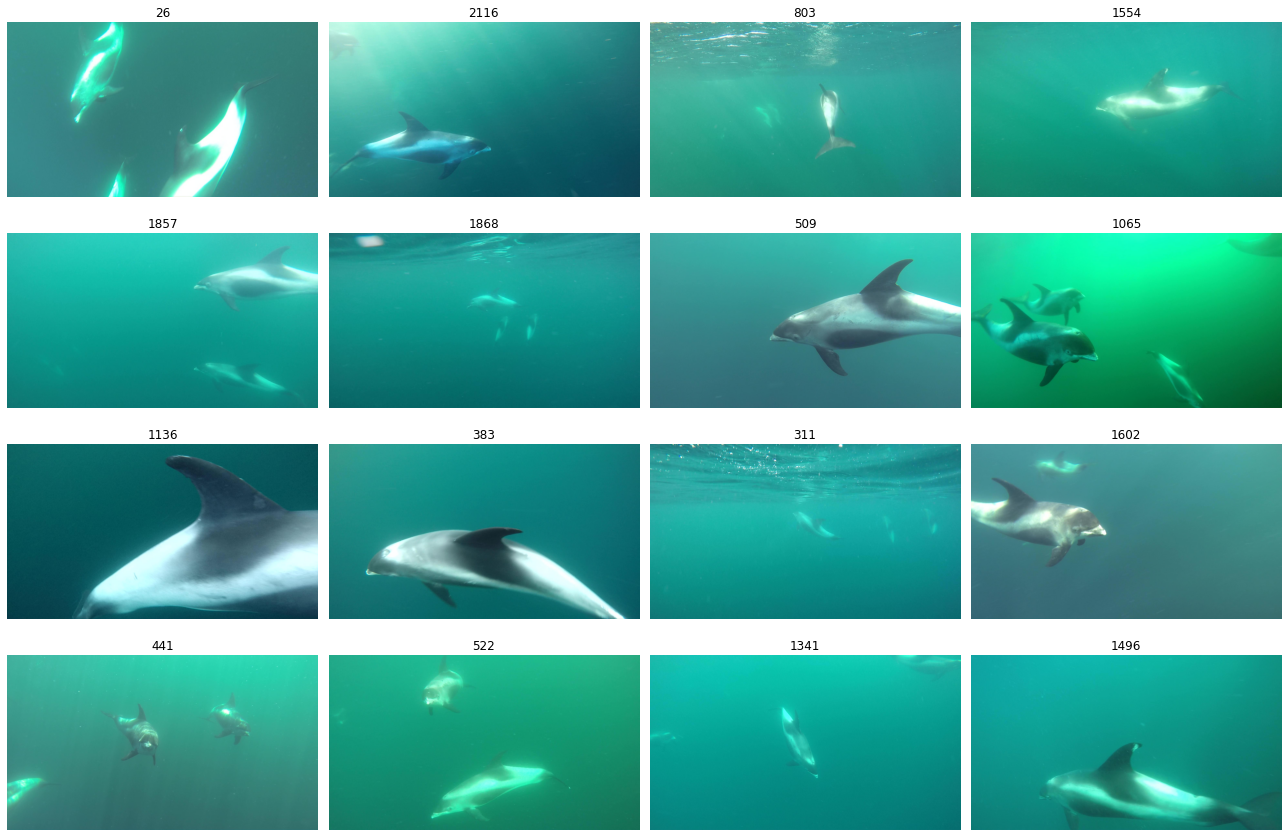
\includegraphics[scale=0.3]{Chapter4/figs/bweg-tiled.png}
	\end{center}
	\caption{Example below water images from NDD20 with filenames displayed. Class labels for masks in each image are noted in Appendix \ref{app:NDD20BwegLabels}.}
	\label{fig:below-water-example}
\end{figure}

\subsection{NDD20 Summary}\label{ch:NDD,sec:NDD20,sub:NDD20Summary}

As NDD20 is split into two related but distinct sets of images, a summary is provided below for each. Due to the nature of cetacean group dynamics, multiple images contain more than one individual animal. As a result, there are 2900 masks present in the above water set of 2201 images. These masks contain both a \texttt{dolphin} label for instance segmentation as well as either a \texttt{BND} or \texttt{WBD} label to facilitate species level fine-grained classification. It should be noted however that the distribution of species class labels is imbalanced, with 73\% of masks being labelled \texttt{BND}. Some above water masks also contain an individual level \texttt{ID} label to allow for extreme fine-grained classification. Due to the nature of the task only 14\% of masks contain an \texttt{ID} class label, with 44 distinct individuals present. Once again these classes are imbalanced presenting both a fine-grained and few-shot learning problem. The above water \texttt{ID} class label distribution can be seen in Figure \ref{fig:above-water-id-dist}. Many of the challenges associated with manual above water photo-id apply here too, particularly the likelihood that unique features are specific to one side of an animal's body which may not have been captured in the image.

\begin{figure}
	\begin{center}
		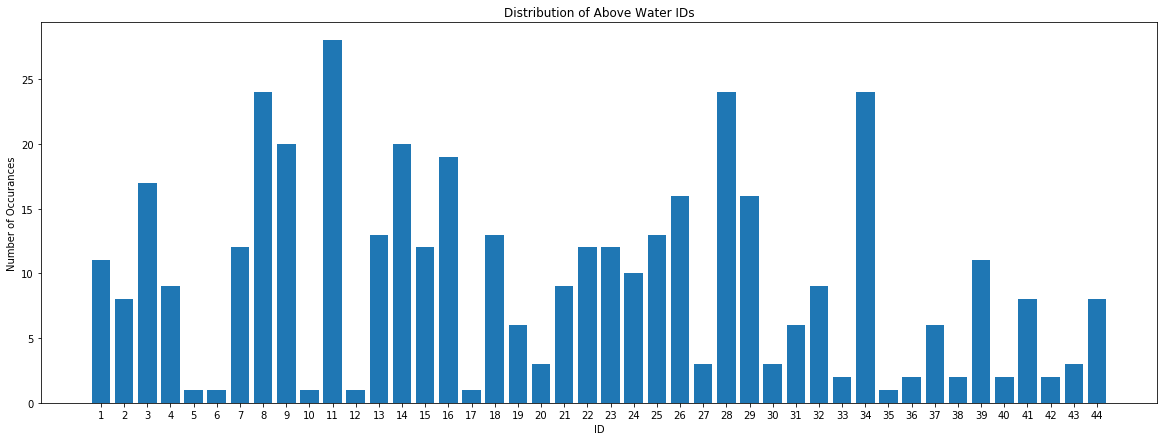
\includegraphics[scale=0.35]{Chapter4/figs/aboveWaterIDDist.png}
	\end{center}
	\caption{The \texttt{ID} class label distribution for the above water set of NDD20.}
	\label{fig:above-water-id-dist}
\end{figure}

Like its above water counterpart, the below water set also contains 2201 images each with at least one mask containing  a \texttt{dolphin} label. Masks in the below water set are significantly larger than in the above water set, as far more of the cetacean is visible when captured below the waterline. Unlike the above water set however, all below water images also contain at least one mask with an \texttt{ID} class label, with 82 classes represented. The distribution of \texttt{ID} class labels in the below water set can be seen in Figure \ref{fig:below-water-id-dist}. This set represents a significantly more challenging fine-grained and few-show learning problem, both due to the higher number of classes as well as decreased image quality thanks to the nature of underwater photography. The main challenges are water clarity, affected by factors such as algae bloom and sunlight refraction which may both obscure areas of the individual useful for identification or add artificial markings which may hinder this. 

\begin{figure}
	\begin{center}
		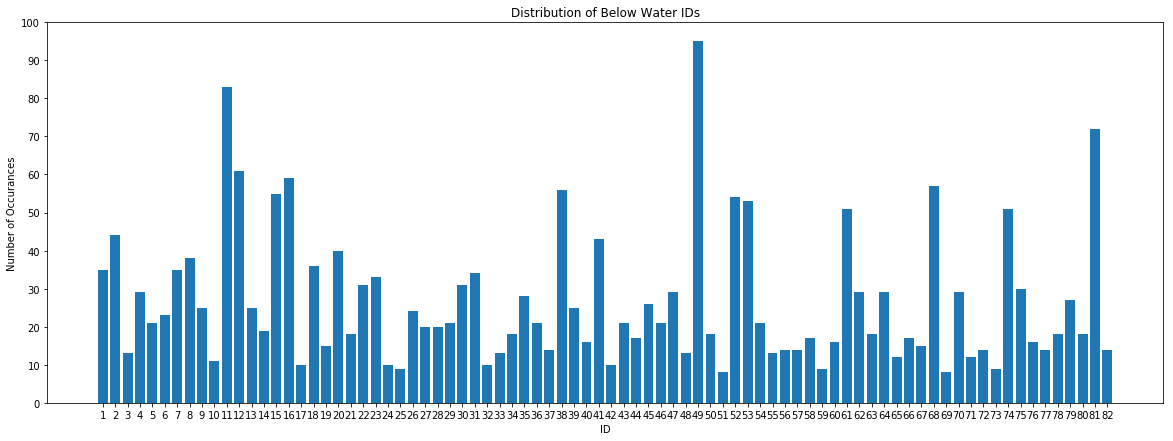
\includegraphics[scale=0.35]{Chapter4/figs/belowWaterIDDist.png}
	\end{center}
	\caption{The \texttt{ID} class label distribution for the below water set of NDD20.}
	\label{fig:below-water-id-dist}
\end{figure}

NDD20 is small compared to traditional benchmarking computer vision datasets such as ImageNet \cite{deng_imagenet:_2009} or those which are domain specific such as iWildcam \cite{beery_iwildcam_2019} or Caltech-UCSD Birds 200 \cite{welinder_caltech-ucsd_2010}. Even when compared to other related non-benchmark marine conservation datasets such as The Fishnet Open Images dataset \cite{kay_fishnet_2021}, SEAMAPD21 \cite{boulais_seamapd21_2021}, or FathomNet \cite{katija_fathomnet_2022}, the number of images in NDD20 is much lower. Whilst it may be tempting to solely compare NDD20 to the above datasets however, it is important to note the difference in use-case. NDD20 is not designed for use as a large scale dataset for model pre-training like those considered benchmark. In contrast to the non-benchmark conservation datasets mentioned, NDD20 contains class labels which allow for more fine-grained classification. As such, it is better to compare the quality of NDD20 with other individual animal identification datasets.

\begin{table}
	\caption[A comparison of computer vision datasets capable of training models for individual animal identification, sorted by number of individuals.]{A comparison of computer vision datasets capable of training models for individual animal identification, sorted by number of individuals.}\label{tab:animal-id-datasets-comparison}
	\begin{adjustbox}{width=\columnwidth, center}
		\begin{tabular}{*{4}{c}}
			\toprule
			\textbf{Dataset}                                                                                                                         & \textbf{Species}                                                                                                & \textbf{Number of Images} & \textbf{Number of Individuals}  \\
			\midrule
			Beluga ID 2022$^\dagger$ & Beluga whale (\textit{Delphinapterus leucas})                & 5902                      & 788                         \\
			Leopard ID 2022$^\ddagger$ & African leopard (\textit{Panthera pardus})                   & 6795                      & 430                         \\
			Hyena ID 2022$^\mathsection$  & Spotted hyena (\textit{Crocuta crocuta})                      & 3104                      & 256                         \\
			Cows2021 \cite{gao_towards_2021}                                                                                                         & Holstein-Friesian cow (\textit{Bos taurus taurus})    & 10,402                     & 186                         \\
			BearID \cite{clapham_automated_2020}                                                                                                     & Brown bear (\textit{Ursus arctos})                            & 4675                      & 132                         \\
			Multi Camera Pig Tracking \cite{shirke_tracking_2021}                                                                                    & Domestic pig (\textit{Sus scrofa domesticus})                 & 380                       & 33                          \\
			Jaguar ID \cite{timm_large-scale_2018}                                                                                                   & Jaguar (\textit{Panthera onca})                               & 176                       & 16                          \\\midrule
			\textbf{NDD20 (Below Water)}                                                                                                                      & White-beaked dolphin (\textit{Lagenorhynchus albirostris})    & 2201                      & 82                         \\
			\multirow{2}{*}{\textbf{NDD20 (Above Water)}}                                                                                                    & Bottlenose dolphin (\textit{Tursiops truncatus})              & \multirow{2}{*}{2201}     & \multirow{2}{*}{44}         \\
			& \& white-beaked dolphin (\textit{Lagenorhynchus albirostris}) &                           &                             \\
			\bottomrule
		\end{tabular}
	\end{adjustbox}

	{\raggedright\footnotesize $\dagger$ Beluga ID 2022: \href{https://lila.science/datasets/beluga-id-2022/}{lila.science/datasets/beluga-id-2022} \\ $\ddagger$ Leopard ID 2022: \href{https://lila.science/datasets/leopard-id-2022/}{lila.science/datasets/leopard-id-2022} \\$\mathsection$ Hyena ID 2022: \href{https://lila.science/datasets/hyena-id-2022/}{lila.science/datasets/hyena-id-2022} \par}
\end{table}

Unlike other datasets for individual animal identification, NDD20 is unusual in that it covers multiple species. Other conservation datasets which cover a range of species do not include individual identification labels \cite{beery_iwildcam_2019, van_horn_inaturalist_2018, khosla_novel_2011}. This combination of multiple species and individual class labels provides novelty to NDD20.

As seen in Table \ref{tab:animal-id-datasets-comparison}, whilst NDD20 is not the smallest dataset available for individual animal identification it is still on the lower end both in terms of number of images and individuals. This is due to the nature of the populations surveyed. The Coquet to St. Mary's and Farnes Deep MCZs are small geographic areas, resulting in smaller population catalogues. The size of the dataset has not limited scientific value however. NDD20 was accepted for presentation at the Fine Grained Visual Categorization workshop at CVPR 2020 \cite{trotter_ndd20_2020}. To coincide with this presentation, the dataset was made public\footnote{NDD20 download: \href{https://doi.org/10.25405/data.ncl.c.4982342}{doi.org/10.25405/data.ncl.c.4982342}}. Furthermore, NDD20 was utilised as one of multiple datasets for use in a Kaggle competition hosted by HappyWhale \footnote{Kaggle competition: \href{https://www.kaggle.com/c/happy-whale-and-dolphin/}{kaggle.com/c/happy-whale-and-dolphin}}. This highlights the usefulness of NDD20 irrespective of size limitations. 


\section{Evaluation Using NDD20}\label{ch:NDD,sec:EvalUsingNDD20}

Once NDD20 had been created it could then be utilised to evaluate the effect of changes in geography, time, and species on the Mask R-CNN based fin detector, as outlined in this Section.

\subsection{Evaluating the Effect of Geography, Time, and Species Change}\label{ch:NDD,sec:EvalUsingNDD20,subsec:geographyTimeSpeciesChange}

As discussed in Chapter \ref{ch:cetDet}, a Mask R-CNN model capable of above water cetacean detection was trained on indo-pacific bottlenose dolphin data collected in Zanzibar, Tanzania. One important requirement of the detector created is that it must be robust enough to output detection masks with high mean average precision (mAP) when operating on data from a different geographic or temporal area without re-training. The creation of NDD20 provides a valuable opportunity to test this requirement. Not only was the data collected in a different location and time, but both species of data subject (bottlenose and white-beaked dolphin) are not present in the Zanzibar dataset.  

To test this requirement the best performing model found on the Zanzibar data in Section \ref{ch:cetDet,sec:ModelSelection,sub:ModelSelectionBasedOnGridSearch}, 20190902T0946, was utilised to generate instance segmentation mask predictions for the above water set of NDD20. These model outputs were then evaluated against the labelled ground truth data to produce an mAP score over multiple IOU thresholds. The results of this evaluation can be seen in Figure \ref{fig:aw-mAP-IOU}.

\begin{figure}
	\begin{center}
		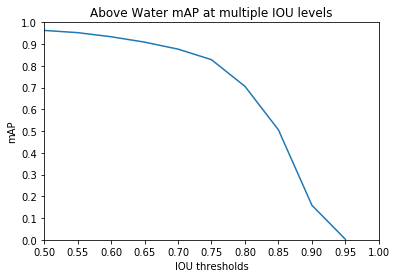
\includegraphics[scale=0.7]{Chapter4/figs/aw-mAP-IOU.png}
	\end{center}
	\caption{mAP@IOU[0.5:0.95] scores for NDD20 using model 20190902T0946 trained on the Zanzibar data.}
	\label{fig:aw-mAP-IOU}
\end{figure}

Model 20190902T0946 still achieves a high mAP at multiple IOU thresholds without the need for re-training or fine-tuning on NDD20. Utilising the same evaluation thresholds as during model selection in Section \ref{ch:cetDet,sec:ModelSelection,sub:ModelSelectionBasedOnGridSearch}, the model achieves mAP@IOU[0.5, 0.75] = [0.96, 0.83] on NDD20. This is in comparison to mAP@IOU[0.5, 0.75] = [0.91, 0.79] on the Zanzibar data. Interestingly, the model achieves a higher mAP at these IOU thresholds on NDD20. This is hypothesised to be due to the lack of other large objects in NDD20 in comparison to the Zanzibar data. For example, some images in the Zanzibar dataset contain other vessels as well as humans as a result of the data being captured in an area with high levels of eco-tourism \cite{christiansen_effects_2010}. This is not the case for data contained within NDD20. Whilst eco-tourism is present in and around the Coquet to St. Mary's MCZ, the levels are significantly lower than in Zanzibar. The evaluated model has been seen to struggle when presented with images containing tourist activity, shown in Figure \ref{fig:model-fail-boat}. As NDD20 lacks this, the model's false positive rate may be reduced. Regardless, this evaluation presents evidence that model 20190902T0946 is robust enough to deal with data from a different geographic area, time, and cetacean species without the need for re-training or fine-tuning. This suggests the model could be deployed to aid in the speed up of future photo-id fieldwork seasons undertaken by conservationists. 

\subsection{Below Water Detection Baseline}\label{ch:NDD,sec:EvalUsingNDD20,subsec:belowWaterDetectionBasleine}

Work was also undertaken to produce a baseline instance segmentation score for the below water set of NDD20. Here, a second Mask R-CNN model was trained using only the below water data divided into an 80:20 train-test split, with the \texttt{out of focus} flag ignored. This model achieved mAP@IOU[0.5, 0.75] = [0.97, 0.91], indicating a Mask R-CNN model is capable of accurate instance segmentation regardless of larger variation in the shape of masks in the below water data as a result of the underwater cameras being able to capture the individual cetaceans in a wider range of movement, as well as there being less differentiation between the background and the individual due to water conditions. The full range of mAP@IOU values can be seen in Figure \ref{fig:bw-mAP-IOU}.

\begin{figure}
	\begin{center}
		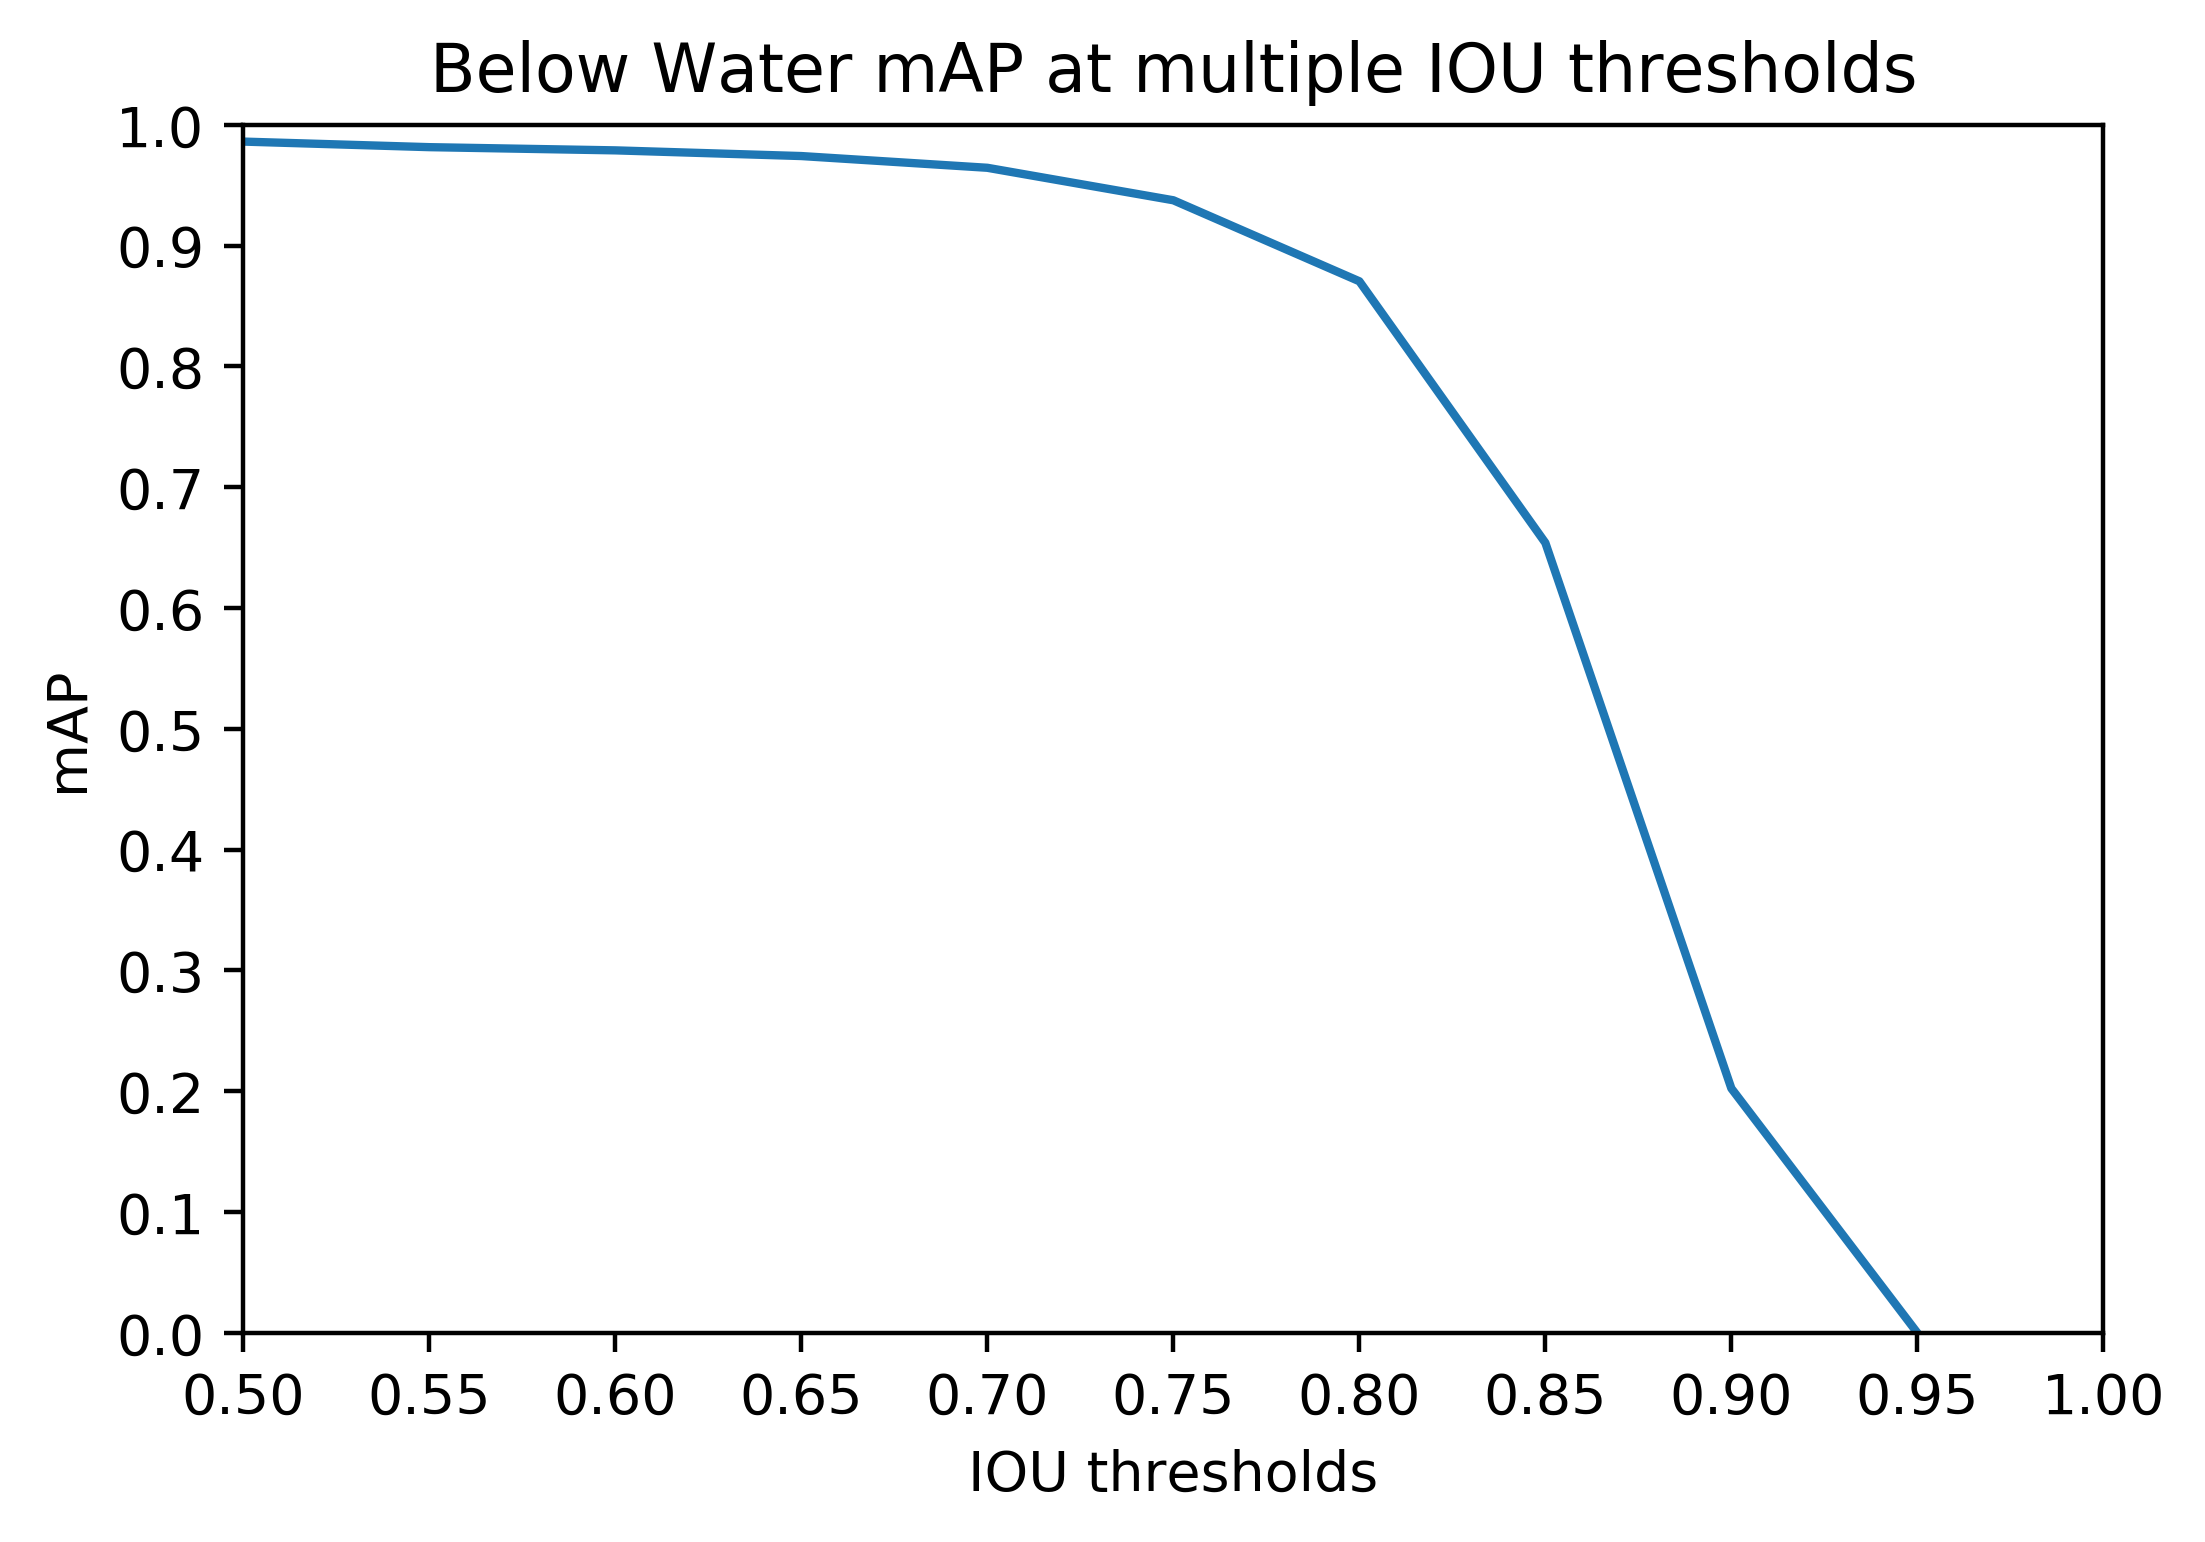
\includegraphics[scale=0.7]{Chapter4/figs/bw-mAP-IOU.png}
	\end{center}
	\caption{Differing mAP@IOU values for the best performing instance segmentation model using the below water data.}
	\label{fig:bw-mAP-IOU}
\end{figure}

\section{Post-Processing NDD20}\label{ch:NDD,sec:postProcessingNDD20}

NDD20 consists of large scale panoramic images, similar to the Zanzibar data before post-processing. As a result, there is a high amount of noise present in the images which should be ignored and removed before the dataset is utilised for individual identification. Whilst Chapter \ref{ch:ID} will focus on both the theory behind, and implementation of, a model capable of individual identification, this Section will detail the processing of NDD20 into a form usable for the task of individual identification.

Utilising the post-processing techniques as outlined in Section \ref{ch:cetDet,sec:postProcessing}, the detections from the Mask R-CNN model were used to generate a dataset of images to train another model capable of individual identification. This dataset, known as \textit{Segmented NDD20}, is a collection of images which contains only the segmented masks from NDD20. 

Once images of the segmentations had been created these were then processed further to create a folder structure which allowed for easy training of an identification model. To facilitate this, each segmentation was checked against the ground truth for the image it was produced from. Any images which contained a dorsal fin with identifying information were placed in a directory containing other examples of that individual. Any fins that did not contain identifying information were removed as their identity could not be guaranteed. Noise which had passed through the mask post-processing were included in a \texttt{noise} directory with the goal of allowing any future model to learn how to identify erroneous masks which have made it through post-processing. 

Example images from Segmented NDD20 are shown in Figure \ref{fig:segmented-ndd20-example}. As can be seen there is low inter-class but high intra-class differences. For example there is relatively little difference between the images shown for individuals \texttt{32} and \texttt{39}, whilst there is a large difference between the three example images for individual \texttt{11}. It is this variance and fine-grained nature which makes the task of automatic individual photo-identification particularly challenging. 

\begin{figure}
	\begin{center}
		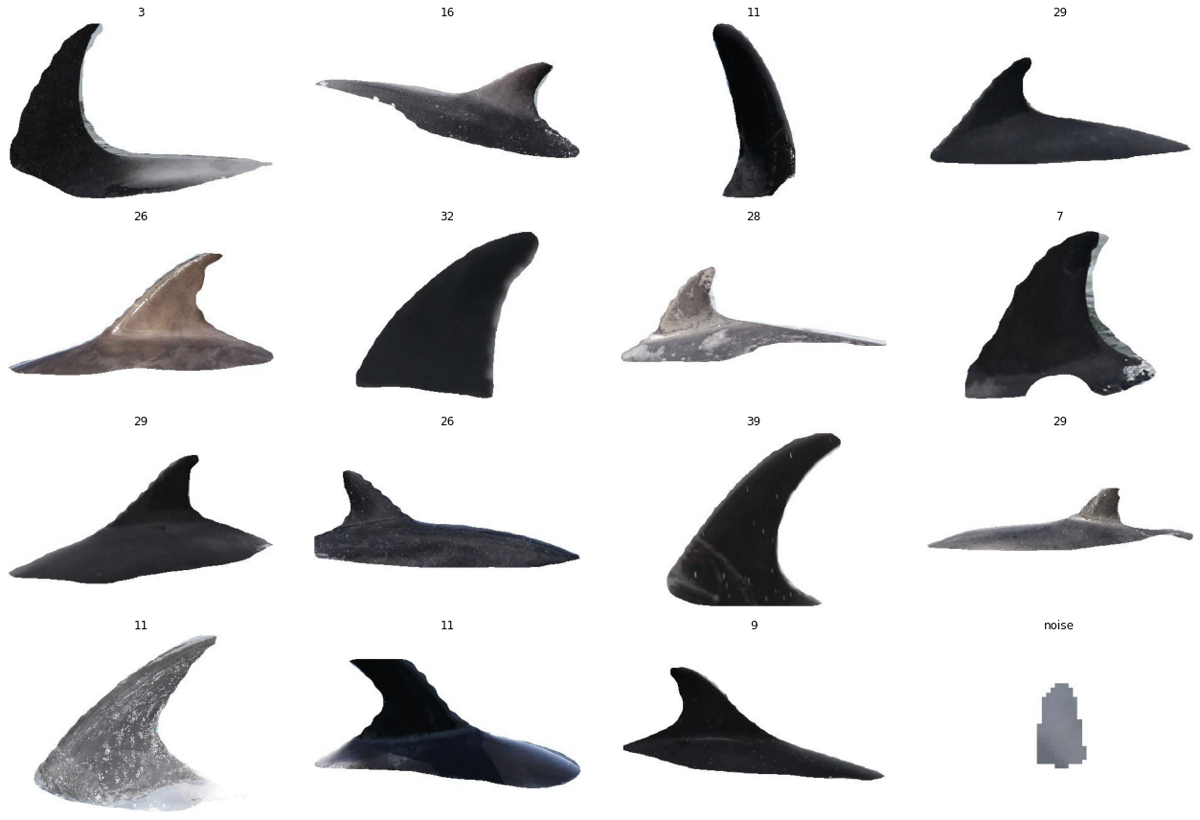
\includegraphics[scale=0.6]{Chapter4/figs/segmented-ndd20-tiled.png}
	\end{center}
	\caption{Example images from Segmented NDD20. The individual class label is displayed above each image.}
	\label{fig:segmented-ndd20-example}
\end{figure}

In total, Segmented NDD20 contains 1243 images representing 43 classes including \texttt{noise}. Individuals \texttt{6} and \texttt{27} were removed from the dataset by the post-processing algorithm. Upon examination, images of these individuals were captured from extreme angles or with large amounts of splash, making it difficult for the detector to produce accurate segmentations. The dataset is highly skewed, as seen in Figure \ref{fig:segmented-ndd20-and-ndd20-au-smru-dist} (blue), with approximately 66\% of images in the dataset labelled as \texttt{noise}. Classes representing individual animals contain a non-uniform number of example images (median = 8.5) varying between 33 examples for individual \texttt{11} to just one for individuals \texttt{5} and \texttt{35}. As such this dataset represents not just a fine-grained but also a few-shot problem, a combination which is extremely challenging for current computer vision methods. 

\begin{figure}
	\begin{center}
		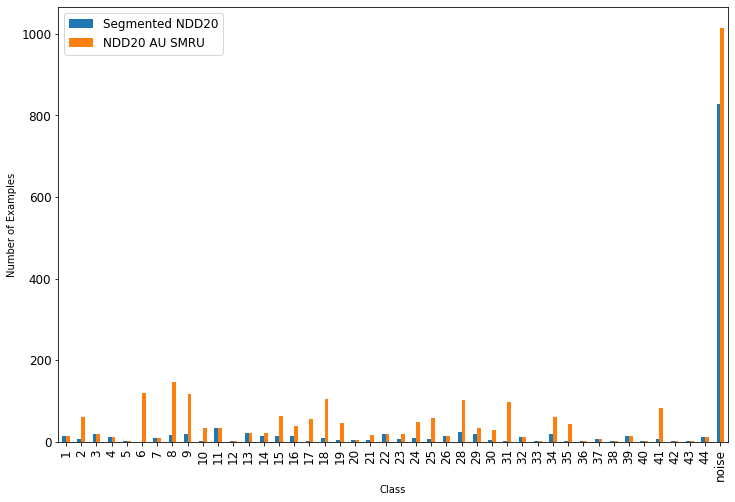
\includegraphics[scale=0.5]{Chapter4/figs/seg-ndd20-and-ndd20-au-smru-dist}
	\end{center}
	\caption{The \texttt{ID} class label distribution for Segmented NDD20 and NDD AU SMRU.}
	\label{fig:segmented-ndd20-and-ndd20-au-smru-dist}
\end{figure}

\section{Additional External Data}\label{ch:NDD,sec:NDD_AU_SMRU}

After post-processing the data collected during fieldwork into the Segmented NDD20 dataset, it was clear from the class distribution present that it may be beneficial to increase the number of examples per individual, providing a photo-id model more data to learn from. As it was not possible due to sea state conditions to continue data collection in the Coquet to St. Mary's MCZ after 10/10/2019, work was undertaken to procure data from other external sources. 

As a result of the large range traversed by cetaceans \cite{shane_ecology_1986} there was a chance that the individuals catalogued in the MCZ had also been recorded in other areas. The underwater habitat found in the MCZ extends upwards as far as the Moray Firth in Scotland. This, along with the knowledge the animals prefer colder waters, led to the assumption that the animals found in Northumberland would likely also be found in catalogues maintained further north. Examination of photo-id catalogues from the University of Aberdeen, provided after discussions with manager of the University's long-term bottlenose dolphin studies manager Dr. Barbara Cheney, confirmed a catalogue overlap. It was determined that 23 individuals (all bottlenose dolphins) were present in both catalogues. As a result of this analysis, Dr. Cheney provided 1827 additional images of the overlapping individuals to complement Segmented NDD20. Images provided were collected by both the University of Aberdeen and the University of St. Andrews' Sea Mammal Research Unit (SMRU) with the approval of Dr. Monica Arso Civil. These images were captured during surveys undertaken between 2003-2019 and were of the highest quality rating on the scale used by the institutions. All images contained only a single individual. 

The additional external data procured was passed through the Mask R-CNN detector and post-processing algorithm, producing images similar to those already present in Segmented NDD20. The post-processed Aberdeen and SMRU data was combined with Segmented NDD20 to produce \textit{NDD AU SMRU}. This dataset consists of 2626 images, 1383 more than Segmented NDD20, representing 44 classes including \texttt{noise}. Individual \texttt{6}, whilst not present in Segmented NDD20 is accounted for in NDD AU SMRU, however individual \texttt{27} still remains absent. Like Segmented NDD20, NDD AU SMRU is heavily skewed towards \texttt{noise} as seen in Figure \ref{fig:segmented-ndd20-and-ndd20-au-smru-dist} (orange) with 61\% of images labelled as this class. Non-\texttt{noise} classes however now have a median of 22 examples per class, providing a larger number of example images to train an automatic photo-id model from. 

The additional external data procured was passed through the Mask R-CNN detector and post-processing algorithm, producing images similar to those already present in Segmented NDD20. The post-processed Aberdeen and SMRU data was combined with Segmented NDD20 to produce \textit{NDD AU SMRU}. This dataset consists of 2626 images, 1383 more than Segmented NDD20, representing 44 classes including \texttt{noise}. Individual \texttt{6}, whilst not present in Segmented NDD20, is accounted for in NDD AU SMRU however individual \texttt{27} still remains absent. Like Segmented NDD20, NDD AU SMRU is heavily skewed towards \texttt{noise} as seen in Figure \ref{fig:segmented-ndd20-and-ndd20-au-smru-dist} (orange), with 61\% of images labelled as this class. Non-\texttt{noise} classes however now have a median of 22 examples per class, providing a larger number of example images to train an automatic photo-id model from. 

\section{Summary}\label{ch:NDD,sec:summary}

This Chapter discusses the collection of bottlenose and white-beaked dolphin abundance estimate data in the coastal waters which make up the Coquet to St. Mary's MCZ. The data, collected over a three month period during the Summer of 2019, was key for testing the Mask R-CNN based detector created in Chapter \ref{ch:cetDet}. Image data collected during the surveys provided evidence to suggest that the fin detection system is invariant to changes in geography, time, and species of interest. Performance of the Mask R-CNN model on the data from Northumberland was not hindered, resulting in a mAP@IOU[0.5, 0.75] = [0.96, 0.83]. This was achieved without re-training or fine-tuning the model for use with the Northumberland data. 

Further, this Chapter examines the creation of the Northumberland Dolphin Dataset 2020 (NDD20), a fine-grain few-shot computer vision dataset created using the imagery collected during the aforementioned abundance estimate surveys. This dataset is comparable in size to other computer vision datasets aimed at individual animal identification as outlined in Table \ref{tab:animal-id-datasets-comparison} however is unique in the fact that it covers multiple species (both bottlenose and white-beaked dolphins) and provides the ability to identify individuals both above and below the waterline. The usefulness of NDD20 is highlighted through its inclusion in a publicly hosted Kaggle competition\footnote{Kaggle competition: \href{https://www.kaggle.com/c/happy-whale-and-dolphin/}{kaggle.com/c/happy-whale-and-dolphin}} and acceptance to the 7\textsuperscript{th} Fine-Grained Visual Categorization Workshop (FGVC7) hosted at CVPR 2020 \cite{trotter_ndd20_2020}. Baseline results on the below water set of NDD20 are also provided. 

Finally, the Chapter discusses the use of the post-processing methodology outlined in Chapter \ref{ch:cetDet} for the creation of Segmented NDD20, a dataset to be utilised for the training of a neural network capable of individual identification. A second dataset called NDD AU SMRU was created by combining Segmented NDD20 and additional data provided by collaborators at the Universities of Aberdeen and St. Andrews after a cross-catalogue matching process was undertaken, highlighting a 23 individual overlap between the catalogues maintained by Newcastle University and the two collaborating universities.

Thanks to the data collection and dataset creation outlined in this Chapter, evaluation of both the Mask R-CNN based fin detector and post-processing methodology outlined in Chapter \ref{ch:cetDet} has been performed. This evaluation confirms the effectiveness of the model for use in a pipeline of networks to aid in the photo-id process. Furthermore the data collection has both allowed for a cross-catalogue study, indicating a large home range for the bottlenose dolphins which inhabit the MCZ, as well as the creation of a computer vision dataset capable of training a network for individual identification. The creation of said network is examined in detail in Chapter \ref{ch:ID}. 

%%%%%%%%%%%%%%%%%%%
